\section{Findings}

\begin{table}
    \caption{Top two commands with top arguments and aliases}
    \label{tab:command-summary}
    \newcommand{\numx}[1]{{\small (\num{#1})}}
\begin{table}
    \caption{Top two commands with top arguments and aliases}
    \label{tab:command-summary}
    \begin{tabular}{@{}lrll@{}}
        \toprule
                    &           \% &            Arguments &                                                                 Aliases (\%) \\
        \midrule
         \verb|git| &   \num{5.85} &        \verb|status| &                              \verb|gs| \numx{54.27}, \verb|gst| \numx{19.19} \\
                    &   \num{3.48} &              \verb|| &                                \verb|g| \numx{75.71}, \verb|gti| \numx{5.74} \\
                    &   \num{3.20} &      \verb|checkout| &      \verb|gco| \numx{50.52}, \verb|gc| \numx{13.87}, \verb|gch| \numx{7.56} \\
                    &   \num{3.18} &          \verb|push| &      \verb|gp| \numx{46.73}, \verb|gps| \numx{9.23}, \verb|push| \numx{7.56} \\
                    &   \num{3.16} &          \verb|diff| &                                                       \verb|gd| \numx{79.89} \\
                    &   \num{2.86} &          \verb|pull| &      \verb|gpl| \numx{18.30}, \verb|gl| \numx{16.59}, \verb|gp| \numx{15.07} \\
                    &   \num{2.78} &        \verb|branch| &                               \verb|gb| \numx{73.54}, \verb|gbr| \numx{6.57} \\
                    &   \num{2.71} &           \verb|add| &                                                       \verb|ga| \numx{80.96} \\
                    &   \num{2.00} &        \verb|commit| &                               \verb|gc| \numx{63.16}, \verb|gci| \numx{5.33} \\
                    &   \num{1.96} &     \verb|commit -m| &       \verb|gcm| \numx{31.29}, \verb|gc| \numx{25.18}, \verb|gm| \numx{7.97} \\
        \midrule
          \verb|ls| &  \num{14.45} &  \verb|--color=auto| &                                                       \verb|ls| \numx{99.04} \\
                    &   \num{8.63} &            \verb|-A| &                                                       \verb|la| \numx{97.61} \\
                    &   \num{7.80} &           \verb|-CF| &                                                        \verb|l| \numx{98.75} \\
                    &   \num{6.78} &          \verb|-alF| &                                                       \verb|ll| \numx{97.49} \\
                    &   \num{5.46} &            \verb|-l| &                                 \verb|ll| \numx{78.83}, \verb|l| \numx{7.91} \\
                    &   \num{3.75} &              \verb|| &                                \verb|l| \numx{27.90}, \verb|sl| \numx{21.45} \\
                    &   \num{2.88} &            \verb|-G| &                                                       \verb|ls| \numx{96.47} \\
                    &   \num{2.74} &           \verb|-la| &      \verb|ll| \numx{38.42}, \verb|la| \numx{26.87}, \verb|lla| \numx{12.63} \\
                    &   \num{2.67} &            \verb|-a| &                                                       \verb|la| \numx{76.94} \\
                    &   \num{1.92} &           \verb|-al| &         \verb|ll| \numx{49.69}, \verb|la| \numx{12.23}, \verb|l| \numx{8.49} \\
        \bottomrule
    \end{tabular}
\end{table}


\end{table}

\Cref{tab:top-summary} shows the most common alias names, commands, and arguments appearing in alias definitions.
The most common alias name we found is \texttt{ls}, appearing a total number of \num{83782} times, which is \per{3.8} of all alias definitions.
Note that this is \texttt{ls} as an \emph{alias name}, a redefinition of the \texttt{ls} \emph{command}, which appears \num{260156} times (\per{10.27}).
This is a bit less often than \texttt{git}, the most common command, which appears in \num{327786} aliases (\per{12.93}).
The most common argument, across all commands, is \texttt{--color=auto}, appearing \num{153931} times (\per{4.24})

Looking at each part of an alias definition in isolation can only get us so far, as arguments only gain meaning in conjunction with commands and alias names can be identical between users, referring to the same command/argument combination, or indeed can overlap, meaning the same alias name is used differently by different users.
\Cref{tab:command-summary} gives a more informative view for the top two commands, \texttt{git} and \texttt{ls}, showing us the top arguments given with each and the most common alias names by which the command/argument combinations are referred to.
Here we can already identify some of the typical alias use cases.
Looking at \texttt{ls}, we find that aliases are used
to redefine the command with a default argument (\alias{ls}{ls --color=auto});
to shorten a common invocation (\alias{ll}{ls -alF});
and to correct a spelling mistake (\alias{sl}{ls}).
We also notice that in the case of \texttt{git}, most aliases are used for shortening \texttt{git} subcommand invocations (e.g. \alias{gd}{git diff}).

\paragraph*{\bf Characterizing Customization Practices}

To capture the range of patterns and use cases for which aliases are defined, we applied inductive coding methods on a selected cross-section of the dataset.
Inductive coding is used when conducting exploratory research without prior expectations on themes in the data \cite{thomas:06}.
It is an iterative process between theoretical sampling and comparing data within emerging themes \cite{dey:03}.
We looked at 1381 alias definitions derived in a similar way as \Cref{tab:command-summary}, i.e. the most common aliases for the most common arguments for the most common commands.
In addition, we took a random sample of 200 alias definitions that each occur only once in the dataset to represent the long tail.
Coding was then performed independently by two authors, who labelled each alias definition in the cross-section with descriptive tags, taking the semantics of the commands into account as much as possible.\footnote{The website \url{https://explainshell.com} has been an indispensable resource.}
After a first iteration, the coders compared their labels, consolidating different naming conventions.
In consecutive iterations, the coders identified ways of formalizing the emerged categories, i.e., constructing mechanisms for classifying alias definitions as belonging to certain categories.
The discussion of the formalizations additionally served to establish a better shared understanding.
Ultimately, the coders reached a saturation point at which further coding and analysis did not lead to further insights.

\begin{table}
    \centering
	\caption{Alias types and customization practices}
    \label{tab:practices}
    \begin{table}
	\caption{Customization practices involving shell aliases}
    \label{tab:practices}
    \begin{tabular}{llrr}
        \toprule
        & & \# & \% \\
        \midrule
        \multicolumn{2}{l}{\textsc{Naming}} & & \\
        & Abbreviating Commands     & \num{999999} & 00.00 \\ % & \verb|alias gc='git commit'| \\
        & Describing Actions        & \num{999999} & 00.00 \\ % & \verb|alias download_file='wget -q -O -'| \\
        & Correcting Misspellings   & \num{999999} & 00.00 \\ % & \verb|alias sduo=sudo| \\
        & Bookmarking Locations     & \num{999999} & 00.00 \\
        \midrule
        \multicolumn{2}{l}{\textsc{Changing}} & & \\
        & Substituting Commands     & \num{999999} & 00.00 \\ % & \verb|alias more=less| \\
        & Overriding Defaults       & \num{999999} & 00.00 \\ % & \verb|alias rm='rm -i'| \\ %du -ach | sort -h
        & Colorizing Output         & \num{999999} & 00.00 \\ % & \verb|alias grep='grep --color=always'| \\
        & Elevating Privilege       & \num{999999} & 00.00 \\ % & \verb|alias apti='sudo apt-get install'| \\
        \midrule
        \multicolumn{2}{l}{\textsc{Composing}} & & \\
        & Building Tools            & \num{999999} & 00.00 \\ % & \verb|alias drm='docker rm $(docker ps -a -q)'| \\
        & Transforming Data         & \num{999999} & 00.00 \\ % & \verb|alias mem10='ps auxf | sort -nr -k 4 | head -10'| \\
        & Chaining Subcommands      & \num{999999} & 00.00 \\ % & \verb|alias brewu='brew update && brew upgrade && brew cleanup'| \\
        \bottomrule
        \end{tabular}
\end{table} % TODO: fill in
\end{table}

We identified nine customization practices among three types of aliases:
\textsc{Shortcuts} introduce new names and are often used for \emph{nicknaming commands}, \emph{abbreviating subcommands}, and \emph{bookmarking locations};
\textsc{Modifications} change the semantics of commands by \emph{substituting commands}, \emph{overriding defaults}, \emph{colorizing output}, and \emph{elevating privilege};
and \textsc{Scripts} combine multiple commands, often for the purposes of \emph{transforming data} or \emph{chaining subcommands}.
\Cref{tab:practices} gives a quantitative overview of the prevalence of each of these practices in the dataset.
Any alias can be an expression of multiple customization practices at once, and some practices only occur with certain commands.
\Cref{tab:practices-by-command} breaks down the customization practices by command, counting the number of aliases that a command is involved in (including aliases that redefine the command).

We will now discuss the alias types and customization practices in more detail.

\subsection{Shortcuts}

The most obvious use of an alias is to give a complex expression a short and/or memorable name.
The average length of an alias name is 4.3 characters, whereas the average length of an alias value is 23.7 characters.
If we divide the length of an alias value by the length of the alias name, we get the \emph{compression ratio} of the alias.
For example, the alias \alias{gs}{git status} has a compression ratio of 5.
\Cref{fig:compression} shows the distribution of compression ratios over all aliases in the dataset.
The median compression ratio is 4.25, meaning half of all alias values are at least four times as long as their alias names.
A compression ratio less than 1 indicates an alias name that is longer than the value it aliases.

There are \num{26055} aliases (\per{1.18}) with names longer than their values.
The two longest alias names we found are from joke definitions.
The first is \num{1772} characters long and is comprised of the letter `f' repeated \num{1053} times, followed by the letter `u' repeated 719 times.
It is an alias for the \verb|cat| command with a similarly named file as an argument.
The second longest alias name is a Swedish compound word of \num{131} characters,\footnote{Translating, roughly, to northwestern-glacier-artillery-flight-thrust-simulator-plant-equipment-maintenance-follow-up-systems-discussion-posts-preparation-works.} aliasing the \verb|ls| command.

On the other end of the spectrum, an alias named \texttt{line} echoes \num{23635} dashes, achieving a compression ratio of \num{5911}.
The second highest compression ratio in any alias definition comes from an alias named \verb|BEEP|, which invokes the Linux \verb|beep| utility 9 times in succession, with a combined \num{4471} arguments.
When executed, it appears to play Daft Punk's 2001 instrumental single \emph{Aerodynamic}.

Beyond just compression and expansion of strings, we can see a few distinct practices related to the naming of things.

\paragraph*{\bf Nicknaming Commands}

There are \num{244872} aliases in our dataset (\per{11.11}) that merely give a new name to a command, without adding any arguments, and without the name belonging to a different command (that would be a substitution, see below).
The most often occurring nicknames are \alias{g}{git}, \alias{c}{clear}, \alias{h}{history}, and \alias{v}{vim}.
Almost all (\per{93.03}) of these kinds of aliases introduce a nickname that is shorter than the command they are referring to, and about half (\per{50.58}) introduce a name that is only one or two characters long.

A special case of nicknaming occurs when the new name is a common misspelling of the command.
In this case, the alias acts like an autocorrect mechanism, as in \alias{got}{git}.
While it is easy for the human eye to determine instances of these typographical errors, it is not as straightforward to formalize all different cases and to distinguish them from regular command shortcuts.
We opt for a conservative criterion (potentially underestimating the true extent of the phenomenon) that looks only at aliases whose names are of the same length as their aliased commands, with a string distance measure above an empirically determined threshold.
We surveyed and experimented with different distance measures~\cite{navarro:01} and decided on using the Damerau-Levenshtein algorithm~\cite{damerau:64}.
It is a robust measure that in addition to tracking the number of insertions, deletions, and substitutions between two strings, also captures the transposition of two characters, a common occurrence in misspelled commands.
We computed the distance measure for all applicable aliases, and determined empirically that a distance measure of 2 seems like a good threshold to decide whether or not an alias corrects a misspelling.
We found \num{9195} aliases (\per{0.42}) that serve as autocorrect rules, most commonly involving transposition (\alias{grpe}{grep}), case-sensitivity (\alias{Jupyter}{jupyter}), localization (\alias{pluralise}{pluralize}), and punctuation (\alias{docker-build}{docker\_build}).

%On the flip side, aliases are also used to disable autocorrect mechanisms.
%The Z shell has built-in spelling correction, which can be selectively disabled using the \verb|nocorrect| command.
%There are \num{7326} aliases (\per{0.33}) in our dataset disabling Z shell autocorrection for certain commands, most commonly the filesystem commands \verb|mv|, \verb|mkdir|, \verb|cp| and \verb|rm|.

\begin{figure}
    \centering
    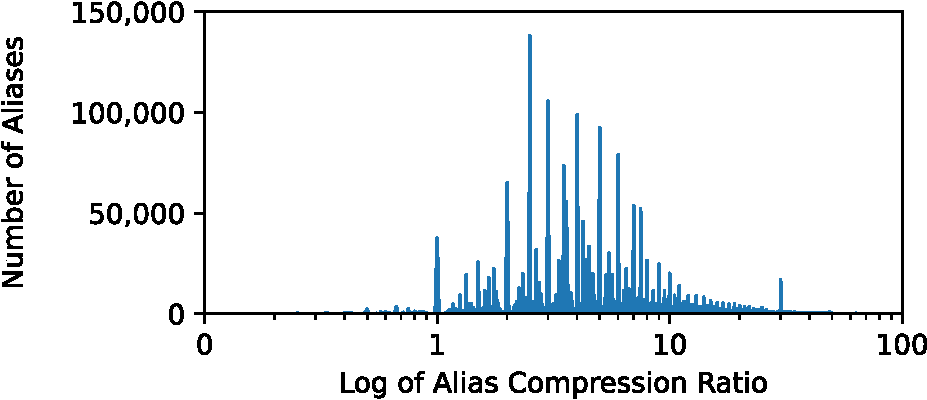
\includegraphics[width=0.95\columnwidth]{figures/compression.pdf}
    \caption{Distribution of alias compression ratios}
    \label{fig:compression}
\end{figure}

\paragraph*{\bf Abbreviating Subcommands}

Many commands can operate in different modes, or act as interfaces to a variety of different \emph{subcommands}.
The subcommand is commonly specified as the first argument to the command, and takes its own set of arguments and flags.
For example, \texttt{git push --tags} executes the \texttt{push} subcommand of \cmd{git} with the \texttt{--tags} flag enabled.
We identified 67 commands in our dataset that take subcommands, such as \cmd{git}, \cmd{docker}, or \cmd{systemctl}.
Noticeably, we found \num{194850} aliases (\per{8.84}) that are purely abbreviations of subcommands, without adding any additional arguments beyond the name of the subcommand.
For example, \alias{gs}{git status} or \alias{gd}{git diff}.
The majority of such subcommand abbreviations (\per{58.5}) are for \cmd{git}, where \num{113980} aliases are defined purely for abbreviating one of its subcommands, accounting for \per{36.77} of all aliases involving \cmd{git}.
The command with the second-most subcommand abbreviations is the package manager \cmd{pacman}, with only \num{9918} instances (\per{5.09} of subcommand abbreviations, but \per{68.67} of all aliases involving \cmd{pacman}).

\paragraph*{\bf Bookmarking Locations}

When an aliased command is called with an argument that references some specific local or remote location, e.g., a file path, domain, or IP address, the alias acts as a bookmark to that location.
For instance, \alias{starwars}{telnet towel.blinkenlights.nl} and \alias{dl}{cd \textasciitilde/Downloads} are both bookmark aliases.

To find such bookmarking uses in our dataset, we searched for arguments that are locations, which we take to be any of the following:
\begin{itemize}
    \item A string containing a forward slash (\verb|/|), indicating a path.
    \item An IPv4 address, matched by the liberal regular expression \verb|[0-9]+.[0-9]+.[0-9]+.[0-9]+|
    \item A string containing one of the known top-level domains\footnote{From \url{http://data.iana.org/TLD/tlds-alpha-by-domain.txt} (retrieved January 14, 2020)} preceded by a dot (\verb|.|) and followed by a slash (\verb|/|), colon (\verb|:|) or the end of the string.
\end{itemize}
To avoid false positives, we sampled the top 300 search results according to the above criteria and determined some exclusion patterns.
For instance, \texttt{/dev/null} is not a location for our purposes.
Neither is \texttt{origin/master}, and thus \alias{gm}{git merge origin/master} does not count as a bookmark.
We also exclude aliases that are merely referencing unnamed relative directories (e.g., \verb|../..|).

By our definition, \num{321546} aliases (\per{14.59}) are bookmarks.
Of these, \num{59931} are remote bookmarks containing URLs or IP addresses (\per{15.92} of all bookmarks).
Bookmarks are used predominantly for file system navigation, and the \verb|cd| command is featured heavily in bookmark aliases.
Most other uses seem to be development related, like starting services such as web servers or databases with pre-defined locations,
or outputting log files, as in \alias{onoz}{cat /var/log/errors.log}, or opening frequently edited files, as in the most common alias for the most common location, which is for editing the shell configuration itself: \alias{zshconfig}{vim \textasciitilde/.zshrc}.
%\Cref{tab:locations} shows the top local and remote locations found in aliases.

% \begin{table}
%     \caption{Top 5 local and remote locations found in aliases}
%     \label{tab:locations}
%     \begin{tabular}{lr}
    \toprule
    Location & \# \\        
    \midrule
    \verb|~/.zshrc|         &   \num{13331} \\
    \verb|~/.bashrc|        &   \num{7319} \\
    \verb|~/.bash_profile|  &   \num{4403} \\
    \verb|~/.vimrc|         &   \num{3612} \\
    \verb|manage.py|        &   \num{2374} \\
    \midrule
    \verb|myip.opendns.com|         &   \num{2670} \\
    \verb|@resolver1.opendns.com|   &   \num{2645} \\
    \verb|8.8.8.8|                  &   \num{706} \\
    \verb|127.0.0.1|                &   \num{643} \\
    \verb|google.com|               &   \num{461} \\
    \bottomrule
\end{tabular}
% \end{table}


\newcommand{\rot}[1]{\makebox[1em][l]{\rotatebox{45}{#1}}}

\newcommand{\full}{$\CIRCLE$}
\newcommand{\half}{$\LEFTcircle$}
\newcommand{\empt}{$\Circle$}

\newcommand{\hist}[1]{\includegraphics[height=1em, trim=1em 1em 1em 1em, clip]{compression/#1.pdf}}

\newcommand*{\pie}[1]{\begin{tikzpicture}[scale=0.15]%
    \draw (0,0) circle (1);
    \fill[fill opacity=1,fill=black] (0,0) -- (90:1) arc (90:90-#1*3.6:1) -- cycle;
    \end{tikzpicture}}

\begin{table*}
    \caption{\TODO}
    \label{tab:practices-by-command}
    \begin{tabular}{llrlllllllllllllccc}
        & & \# & &\rot{Abbreviating Commands} & \rot{Describing Actions} & \rot{Correcting Misspellings} & \rot{Bookmarking Locations} & & \rot{Substituting Commands} & \rot{Overriding Defaults} & \rot{Colorizing Output} & \rot{Elevating Privilege} & & \rot{Building Tools} & \rot{Transforming Data} & \rot{Chaining Subcommands} & & Compression Ratio \\
        \midrule
        \multicolumn{2}{l}{Version Control} \\
            & \texttt{git} & \num{999999} & & \pie{0} & \pie{0} & \pie{0} & \pie{0} & & \pie{0} & \pie{0} & \pie{0} & \pie{0} & & \pie{0} & \pie{0} & \pie{0} & & \hist{git} \\
            & \texttt{hg} & \num{999999} & & \pie{0} & \pie{0} & \pie{0} & \pie{0} & & \pie{0} & \pie{0} & \pie{0} & \pie{0} & & \pie{0} & \pie{0} & \pie{0} & & \hist{hg} \\
        \midrule
        \multicolumn{2}{l}{System Tools} \\
        & \texttt{ls} & \num{999999} & & \pie{0} & \pie{0} & \pie{0} & \pie{0} & & \pie{0} & \pie{0} & \pie{0} & \pie{0} & & \pie{0} & \pie{0} & \pie{0} & & \hist{ls} \\
        & \texttt{cd} & \num{999999} & & \pie{0} & \pie{0} & \pie{0} & \pie{0} & & \pie{0} & \pie{0} & \pie{0} & \pie{0} & & \pie{0} & \pie{0} & \pie{0} & & \hist{cd} \\
        & \texttt{grep}* & \num{999999} & & \pie{0} & \pie{0} & \pie{0} & \pie{0} & & \pie{0} & \pie{0} & \pie{0} & \pie{0} & & \pie{0} & \pie{0} & \pie{0} & & \hist{grep} \\
        & \texttt{echo} & \num{999999} & & \pie{0} & \pie{0} & \pie{0} & \pie{0} & & \pie{0} & \pie{0} & \pie{0} & \pie{0} & & \pie{0} & \pie{0} & \pie{0} & & \hist{echo} \\
        & \texttt{xargs} & \num{999999} & & \pie{0} & \pie{0} & \pie{0} & \pie{0} & & \pie{0} & \pie{0} & \pie{0} & \pie{0} & & \pie{0} & \pie{0} & \pie{0} & & \hist{xargs} \\
        & \texttt{ssh} & \num{999999} & & \pie{0} & \pie{0} & \pie{0} & \pie{0} & & \pie{0} & \pie{0} & \pie{0} & \pie{0} & & \pie{0} & \pie{0} & \pie{0} & & \hist{ssh} \\
        & \texttt{rm} & \num{999999} & & \pie{0} & \pie{0} & \pie{0} & \pie{0} & & \pie{0} & \pie{0} & \pie{0} & \pie{0} & & \pie{0} & \pie{0} & \pie{0} & & \hist{rm} \\
        & \texttt{dir} & \num{999999} & & \pie{0} & \pie{0} & \pie{0} & \pie{0} & & \pie{0} & \pie{0} & \pie{0} & \pie{0} & & \pie{0} & \pie{0} & \pie{0} & & \hist{dir} \\
        & \texttt{cp} & \num{999999} & & \pie{0} & \pie{0} & \pie{0} & \pie{0} & & \pie{0} & \pie{0} & \pie{0} & \pie{0} & & \pie{0} & \pie{0} & \pie{0} & & \hist{cp} \\
        & \texttt{mv} & \num{999999} & & \pie{0} & \pie{0} & \pie{0} & \pie{0} & & \pie{0} & \pie{0} & \pie{0} & \pie{0} & & \pie{0} & \pie{0} & \pie{0} & & \hist{mv} \\
        & \texttt{sort} & \num{999999} & & \pie{0} & \pie{0} & \pie{0} & \pie{0} & & \pie{0} & \pie{0} & \pie{0} & \pie{0} & & \pie{0} & \pie{0} & \pie{0} & & \hist{sort} \\
        & \texttt{head} & \num{999999} & & \pie{0} & \pie{0} & \pie{0} & \pie{0} & & \pie{0} & \pie{0} & \pie{0} & \pie{0} & & \pie{0} & \pie{0} & \pie{0} & & \hist{head} \\
        & \texttt{cat} & \num{999999} & & \pie{0} & \pie{0} & \pie{0} & \pie{0} & & \pie{0} & \pie{0} & \pie{0} & \pie{0} & & \pie{0} & \pie{0} & \pie{0} & & \hist{cat} \\
        \midrule
        \multicolumn{2}{l}{Package Managers} \\
        & \texttt{apt}* & \num{999999} & & \pie{0} & \pie{0} & \pie{0} & \pie{0} & & \pie{0} & \pie{0} & \pie{0} & \pie{0} & & \pie{0} & \pie{0} & \pie{0} & & \hist{apt} \\
        & \texttt{zypper} & \num{999999} & & \pie{0} & \pie{0} & \pie{0} & \pie{0} & & \pie{0} & \pie{0} & \pie{0} & \pie{0} & & \pie{0} & \pie{0} & \pie{0} & & \hist{zypper} \\
        & \texttt{pacman} & \num{999999} & & \pie{0} & \pie{0} & \pie{0} & \pie{0} & & \pie{0} & \pie{0} & \pie{0} & \pie{0} & & \pie{0} & \pie{0} & \pie{0} & & \hist{pacman} \\
        & \texttt{mvn} & \num{999999} & & \pie{0} & \pie{0} & \pie{0} & \pie{0} & & \pie{0} & \pie{0} & \pie{0} & \pie{0} & & \pie{0} & \pie{0} & \pie{0} & & \hist{mvn} \\
        & \texttt{yaourt} & \num{999999} & & \pie{0} & \pie{0} & \pie{0} & \pie{0} & & \pie{0} & \pie{0} & \pie{0} & \pie{0} & & \pie{0} & \pie{0} & \pie{0} & & \hist{yaourt} \\
        & \texttt{brew} & \num{999999} & & \pie{0} & \pie{0} & \pie{0} & \pie{0} & & \pie{0} & \pie{0} & \pie{0} & \pie{0} & & \pie{0} & \pie{0} & \pie{0} & & \hist{brew} \\
        & \texttt{port} & \num{999999} & & \pie{0} & \pie{0} & \pie{0} & \pie{0} & & \pie{0} & \pie{0} & \pie{0} & \pie{0} & & \pie{0} & \pie{0} & \pie{0} & & \hist{port} \\
        \midrule
        \multicolumn{2}{l}{Text Editors}  \\
        & \texttt{mate} & \num{999999} & & \pie{0} & \pie{0} & \pie{0} & \pie{0} & & \pie{0} & \pie{0} & \pie{0} & \pie{0} & & \pie{0} & \pie{0} & \pie{0} & & \hist{mate} \\
        & \texttt{vim} & \num{999999} & & \pie{0} & \pie{0} & \pie{0} & \pie{0} & & \pie{0} & \pie{0} & \pie{0} & \pie{0} & & \pie{0} & \pie{0} & \pie{0} & & \hist{vim} \\
        & \texttt{nvim} & \num{999999} & & \pie{0} & \pie{0} & \pie{0} & \pie{0} & & \pie{0} & \pie{0} & \pie{0} & \pie{0} & & \pie{0} & \pie{0} & \pie{0} & & \hist{nvim} \\
        & \texttt{emacs} & \num{999999} & & \pie{0} & \pie{0} & \pie{0} & \pie{0} & & \pie{0} & \pie{0} & \pie{0} & \pie{0} & & \pie{0} & \pie{0} & \pie{0} & & \hist{emacs} \\
        \midrule
        \multicolumn{2}{l}{Infrastructure} \\
        & \texttt{docker}* & \num{999999} & & \pie{0} & \pie{0} & \pie{0} & \pie{0} & & \pie{0} & \pie{0} & \pie{0} & \pie{0} & & \pie{0} & \pie{0} & \pie{0} & & \hist{docker} \\
        & \texttt{kubectl}* & \num{999999} & & \pie{0} & \pie{0} & \pie{0} & \pie{0} & & \pie{0} & \pie{0} & \pie{0} & \pie{0} & & \pie{0} & \pie{0} & \pie{0} & & \hist{kubectl} \\
        & \texttt{vagrant} & \num{999999} & & \pie{0} & \pie{0} & \pie{0} & \pie{0} & & \pie{0} & \pie{0} & \pie{0} & \pie{0} & & \pie{0} & \pie{0} & \pie{0} & & \hist{vagrant} \\
        \midrule
        \multicolumn{2}{l}{Other} \\
        & \texttt{ffmpeg} & \num{999999} & & \pie{0} & \pie{0} & \pie{0} & \pie{0} & & \pie{0} & \pie{0} & \pie{0} & \pie{0} & & \pie{0} & \pie{0} & \pie{0} & & \hist{ffmpeg} \\
        & \texttt{beep} & \num{999999} & & \pie{0} & \pie{0} & \pie{0} & \pie{0} & & \pie{0} & \pie{0} & \pie{0} & \pie{0} & & \pie{0} & \pie{0} & \pie{0} & & \hist{beep} \\
    \end{tabular}
\end{table*}
 % TODO: update

\subsection{Modifications}

Aliases are not only used syntactically, for naming purposes, but also in ways that change the semantics of certain commands.
We found four customization practices where aliases modify commands.

\paragraph*{\bf Substituting Commands}

When the name of an alias is identical to the name of a pre-existing command, the alias defines a substitution for the command.
A common example is \alias{more}{less}, replacing a standard Unix utility (\cmd{more}) with a more capable but similar command (\cmd{less}).
This can also be used for subterfuge, as in \alias{emacs}{vim} (appearing 132 times in our dataset) or indeed \alias{vim}{emacs} (86 times, alas).

To determine which alias names are also names of actual commands, we compared them to known Unix commands,\footnote{\url{https://en.wikipedia.org/wiki/List_of_Unix_commands} and \url{https://en.wikipedia.org/wiki/List_of_GNU_Core_Utilities_commands}} as well as a curated sample of commands from our dataset (taking care to not include names that appear in a command position but are actually just other aliases).
To determine proper substitutions, we only count aliases whose value does not also include the name of the command (which would point to an overriding alias, see below).
We find that \num{100564} aliases (\per{4.56}) are used to substitute one command for another.
The top three substitutions are \verb|vi| $\rightarrow$ \verb|vim|, \verb|vim| $\rightarrow$ \verb|nvim|, and \verb|vi| $\rightarrow$ \verb|nvim|.

\paragraph*{\bf Overriding Defaults}

When the name of the alias is a pre-existing command that is also part of the alias itself, as in \alias{ls}{ls -G}, then the alias re-defines the command and effectively overrides its default settings.
Any time the command is now executed, it will be with the arguments specified in the alias.
There are \num{319239} aliases in our dataset (\per{14.48}) that are used to override defaults in this way.
Aliases to override the defaults of the \cmd{grep} family of commands (\cmd{grep}, \cmd{egrep}, \cmd{fgrep}) occur \num{96970} times, which is \per{68.27} of all \cmd{grep} appearances and accounts for \per{4.4} of all alias definitions.
The \cmd{ls} command is redefined with new defaults \num{75374} times (\per{28.99} of \cmd{ls} appearances), accounting for \per{3.42} of all aliases.
Also of note are the file system commands \cmd{mv}, \cmd{cp}, and \cmd{rm}, where redefinitions account for \per{89.3}, \per{80.9}, and \per{55.37} of all appearances of these commands, respectively.

Looking in detail at the new defaults of these redefined commands, we find they reveal a variety of user preferences, especially in the diverse long tail, where we find a lot of unique alias definitions and argument combinations.
Two areas of customization stand out, however: formatting output and adding safety.
The majority of overrides for file system commands (\cmd{mv}, \cmd{cp}, and \cmd{rm}, but also \cmd{ln}, for creating symbolic links) are to enable interactive mode (\texttt{-i} and variations), which prompts the user before performing potentially destructive actions.
Verbose output (\texttt{-v}) also plays a role here, describing exactly what kind of effects a command execution had or will have.
Enabling verbosity can also be seen as a kind of output formatting, although much more common is the wish for human-readable output.
For example, the alias \alias{df}{df -h} ensures that the available disk space is displayed in common size units, as opposed to just the raw number of bytes.
But by far the most common reason for overriding defaults is to enable colorized output.
This behavior is so prevalent that we count it as a customization practice in its own right.

\paragraph*{\bf Colorizing Output}

Enabling colored output can be done in many different ways: adding an argument (like \texttt{less -R} or \cmd{grep --color=always}), setting an environment variable (as in \alias{ssh}{TERM=xterm256color ssh}), running the command through a tool that colorizes its output (like \cmd{grcat} or \cmd{pygmentize}), or even replacing a command outright (\alias{diff}{colordiff}).
Taking all these varieties into account, more than half of all command redefinitions (\per{57.21}) enable colored output by default.
This amounts to a surprising \num{182623} aliases, or \per{8.29} percent of all aliases in the dataset.
If we extend this count to also include aliases that introduce new names (like \alias{ll}{ls -l --color=auto}), then more than \per{10} of aliases ensure that a command's output is not just in black and white.

\paragraph*{\bf Elevating Privilege}

The \cmd{sudo} command allows the user to execute another command with superuser privileges.
Combining a command with \cmd{sudo} is often necessary if the other command needs to modify critical parts of the system.
In our dataset, we found \num{93683} aliases (\per{4.25}) in which a command is prefixed with \cmd{sudo}.
The top \cmd{sudo}-prefixed command is the package manager \cmd{apt-get}, appearing \num{10467} times with \cmd{sudo}.
Remarkably, these are \per{89.35} of all occurrences of \cmd{apt-get}.
In fact, \per{72.45} of all occurrences of the package managers \cmd{apt}* (Debian and derivatives; including \cmd{apt}, \cmd{apt-get}, \cmd{apt-cache}, \cmd{aptitude}, and \cmd{\$apt\_pref}), \cmd{pacman}, \cmd{abs} and \cmd{aur} (Arch Linux), \cmd{yum} (RPM), \cmd{dnf} (Fedora), \cmd{zypper} (openSUSE), \cmd{port} (macOS), and \cmd{gem} (Ruby) are together with \cmd{sudo}, and these package managers account for \per{29.1} of all \cmd{sudo} occurrences.
Interestingly, the macOS package manager \cmd{brew} rarely appears with \cmd{sudo} (only \per{1.07}), even though it is the third most occurring package manager overall, behind \cmd{apt}* and \cmd{pacman}.

Other commands that more often than not demand elevated privileges are system utilities like \cmd{systemctl}, \cmd{shutdown}, \cmd{lsof} or \cmd{mount}.

\subsection{Scripts}

Alias values are not limited to single commands and their arguments, but can be arbitrarily complex compositions of multiple commands.
In our dataset, \num{204142} aliases (\per{9.26}) are composed of more than one command.
The most popular way to combine commands is with a pipe (\verb`|`), used by \per{39.66} percent of multi-command aliases, followed by the operators for simple chaining (\verb|;|), with \per{29.61}, and logical conjunction (\verb|&&|), with \per{26.88}.
Other operators (\verb`||`, \verb`|&`) appear in only \per{3.85} of multi-command aliases.

Aliases that combine multiple commands are basically tiny shell scripts.
Two scripting practices are of particular interest.

\paragraph*{\bf Transforming Data}

The most interesting shell operator is certainly the pipe (\verb`|`), since it creates an interface between two otherwise separate programs.
The pipe embodies the Unix philosophy of small tools doing one thing well, which can then be connected together to accomplish more complex tasks.
There are \num{74719} aliases (\per{3.39}) combining two or more commands using only the pipe operator.
The most common command occurring in these pipelines by far is \cmd{grep}, which makes an appearance in almost half of all pipelines (\per{46.16}), more than three times as often as \cmd{xargs} and \cmd{sort}, the next most common commands used for transforming data.
The most common data sources in pipelines are the commands \cmd{ps}, \cmd{git}, and \cmd{ls}, which can be found at the beginning of almost a third (\per{32}) of all pipelines.
\Cref{fig:flow} shows a flow diagram of the top 250 pipelines with three commands that make up at least \per{10} of one participating command's usage.

\begin{figure*}[h]
	\centering    
	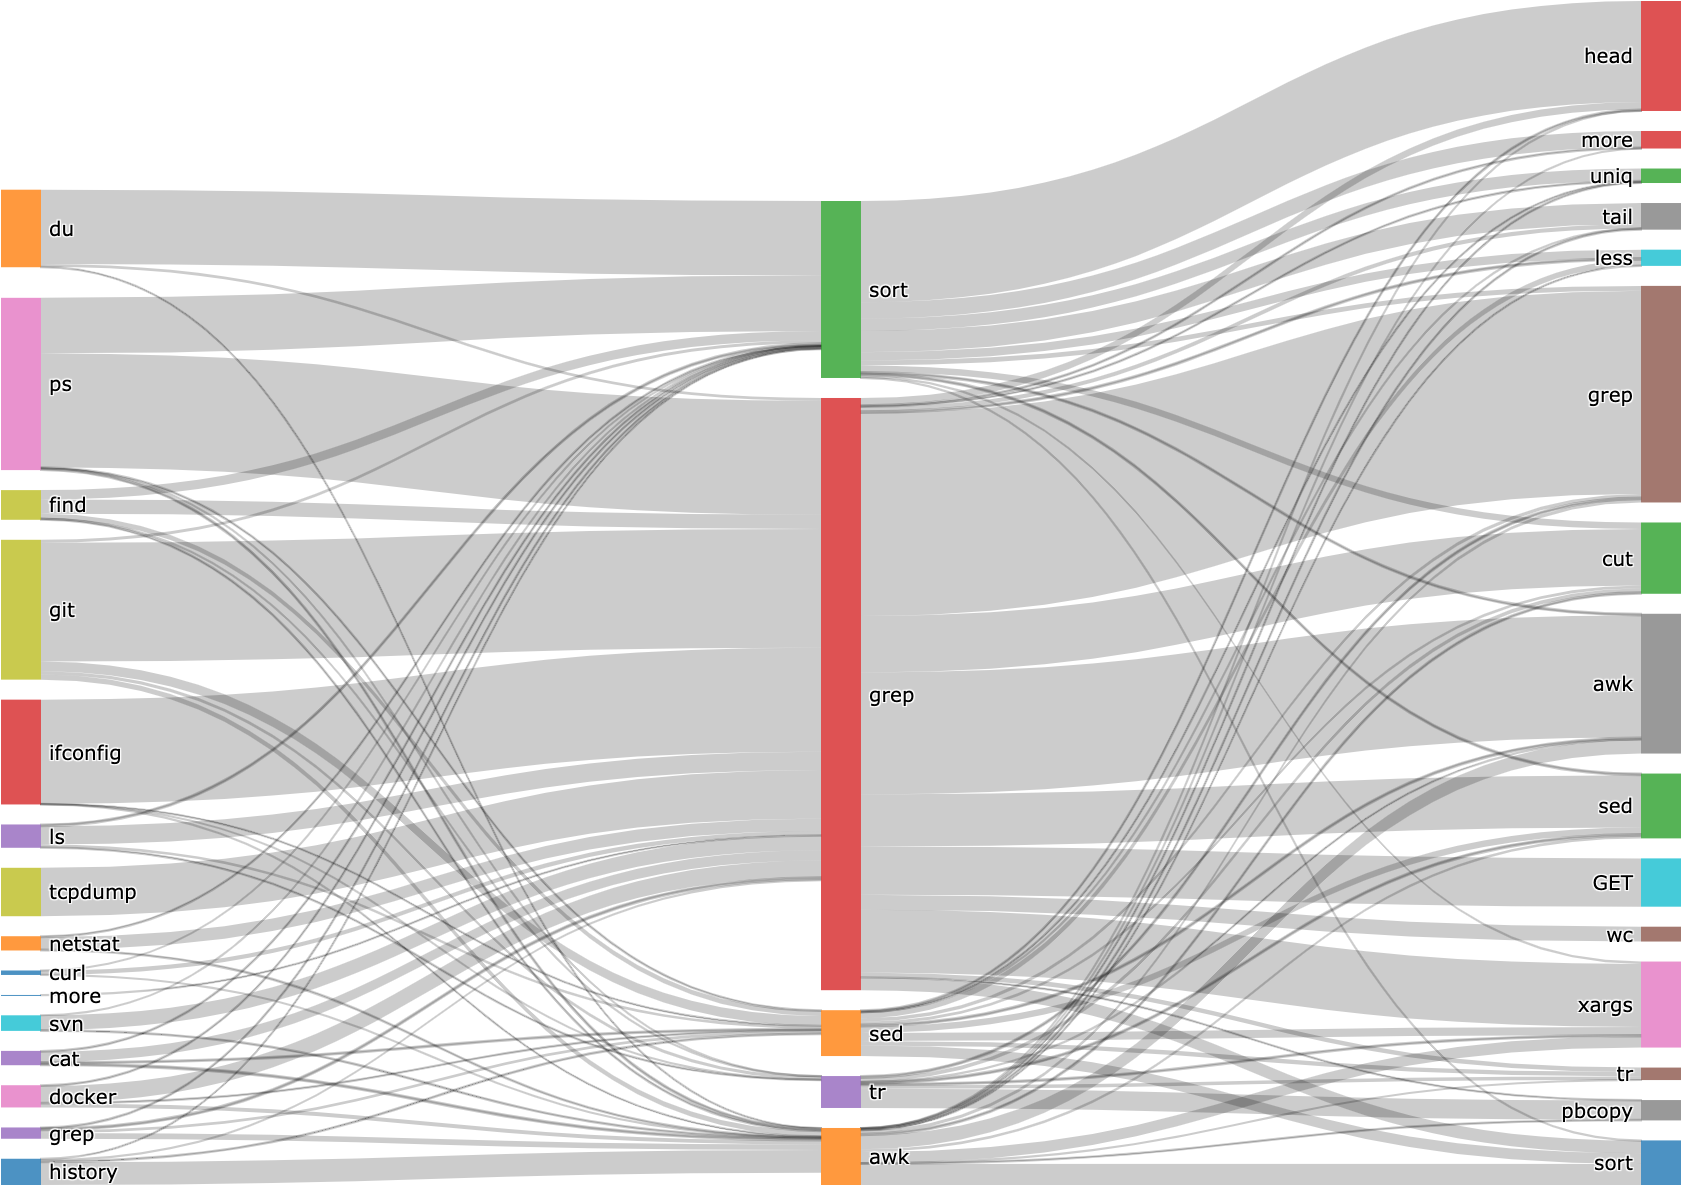
\includegraphics[width=0.78\linewidth]{figures/flow_250.png}
	\caption{Flow diagram for top 3-command pipelines}
	\label{fig:flow}
\end{figure*}

\paragraph*{\bf Chaining Subcommands}

An interesting pattern found in aliases composed of multiple commands are chains of subcommand invocations.
For example, the package manager \cmd{brew} has a subcommand \texttt{update}, for updating the package database, and a subcommand \texttt{upgrade}, for upgrading previously installed packages to the latest available versions.
\per{28.08} percent of all aliases involving the \cmd{brew} command contain the composition
\begin{CVerbatim}
brew update && brew upgrade
\end{CVerbatim}
(sometimes with \verb|;| instead of \verb|&&|), with alias names like \verb|update|, \verb|brewup|, \verb|bup|, etc.
This pattern of repeated subcommand invocations can be found in \num{22062} aliases (\per{1}), and it is most prevalent among package managers, like \cmd{brew}, \cmd{apt-get}, \cmd{npm} or \cmd{gem}, mostly fulfilling roughly the same function as in the \cmd{brew} example.

The command with the highest absolute number of aliases showing this pattern is \cmd{git}, however, with \num{12063} occurrences (\per{3.89} of all aliases using \cmd{git}).
Here, the uses are more varied, 
e.g., \alias{commit}{git add . \&\& git commit -m}, 
or \alias{gitpull}{git stash \&\& git pull \&\& git stash pop},
or indeed \alias{whoops}{git reset --hard \&\& git clean -df}.
